\chapter{Revealed Subsets}
\label{app:subsets}

In the main text, we present figures outlining for a given budget, what percentage of budgets of a given size were selected by each algorithm for a given budget.
Here, for completeness, we offer more detailed figures, showing what subsets were actually selected.

\begin{figure*}[t!]
  \centering
	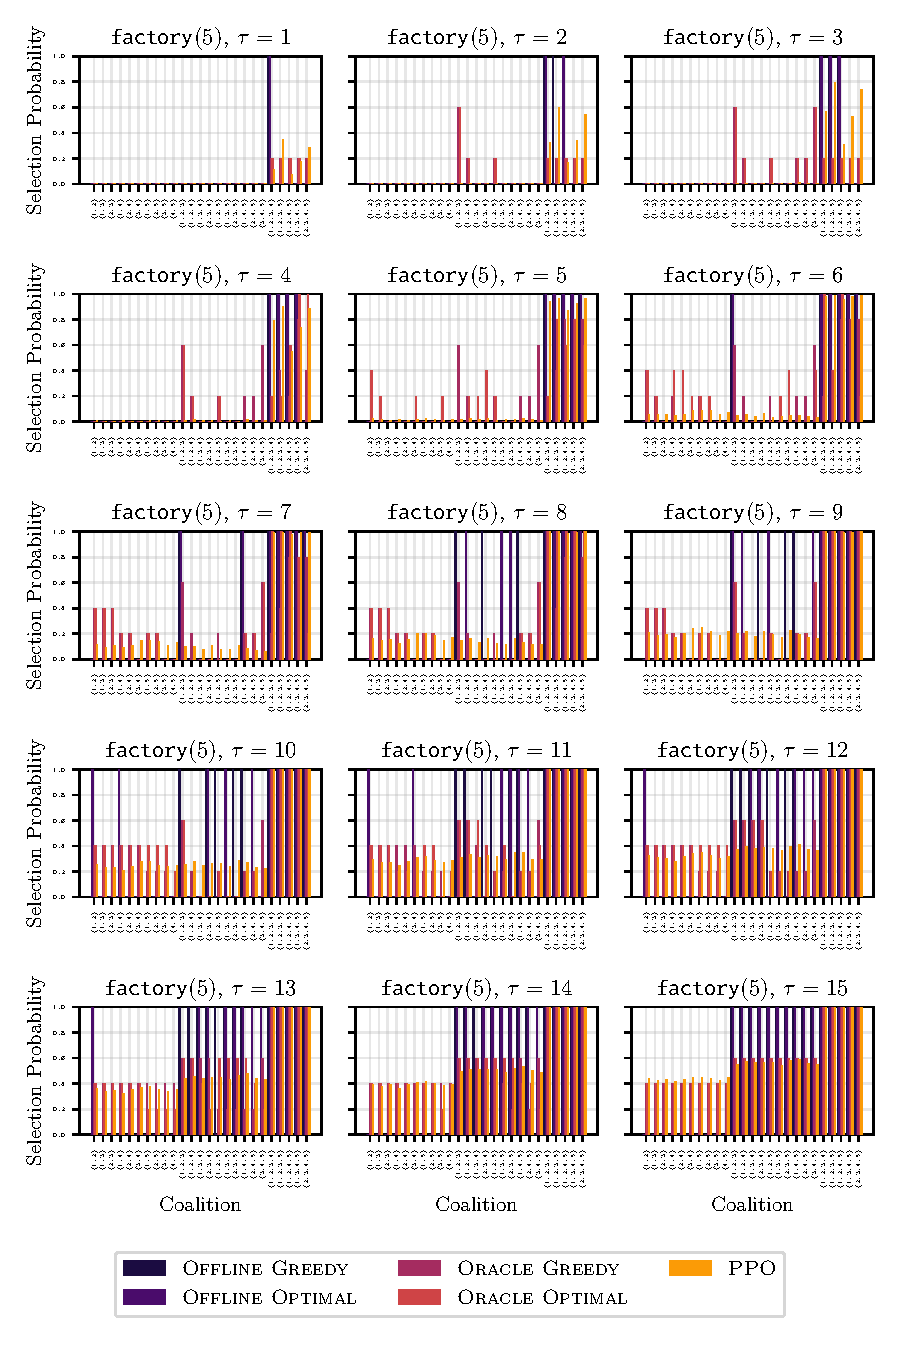
\includegraphics[width=\textwidth]{figures/exploitability_predictible_factory5_coalition_bars.pdf}
	\caption{ The probability of revealing a given subset for $\tau=1\ldots 15$ for the different approaches, when ran on the $\factory[5]$ distribution with the utopian gap. 
		The resulting utopian gap can be seen in \Cref{fig:factory}.
	}
\end{figure*}

\begin{figure*}[t!]
  \centering
	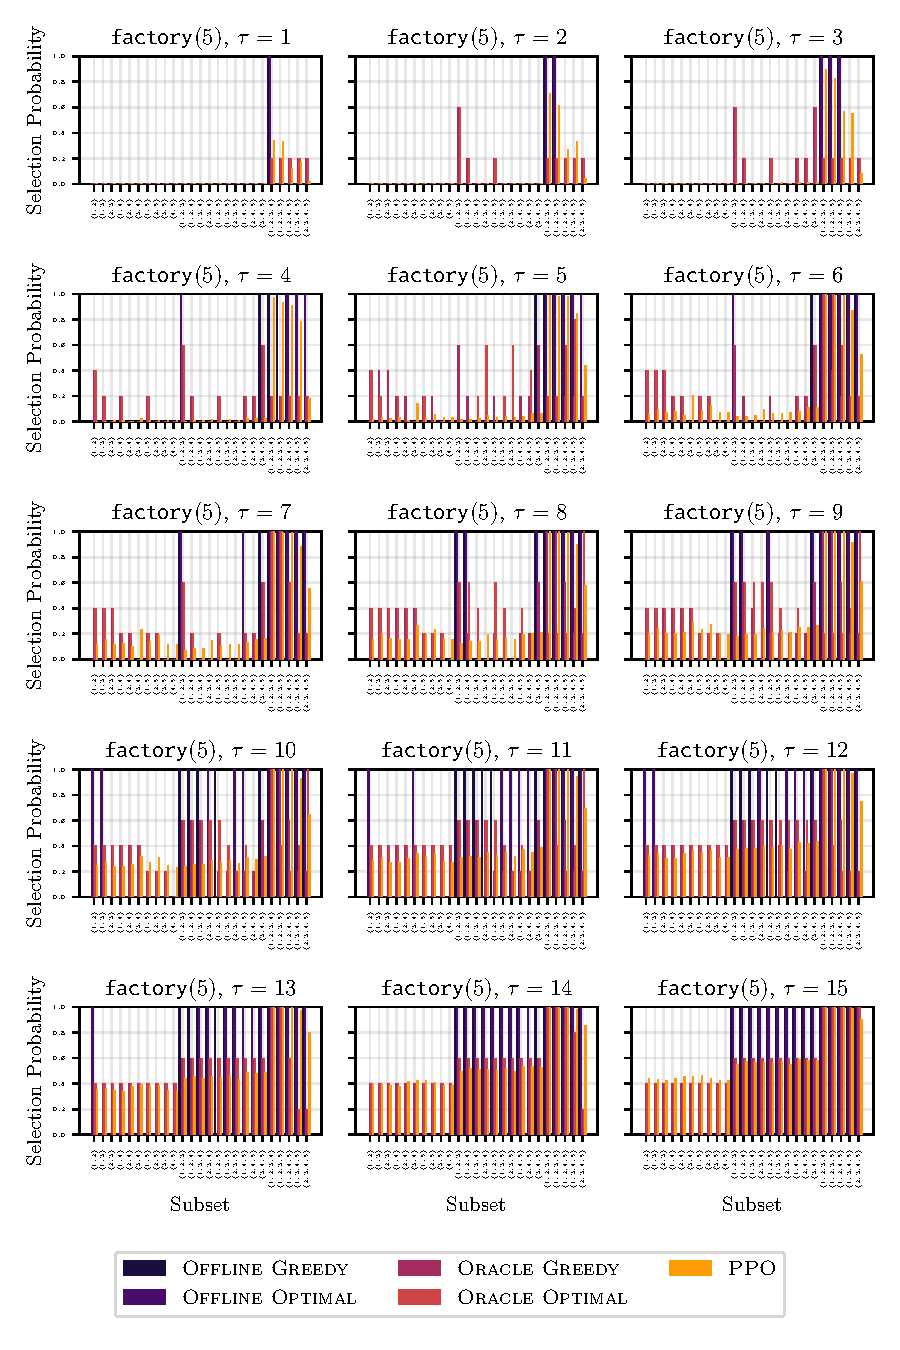
\includegraphics[width=\textwidth]{figures/l1_norm_predictible_factory5_coalition_bars.pdf}
	\caption{ The probability of revealing a given subset for $\tau=1\ldots 15$ for the different approaches, when ran on the $\factory[5]$ distribution with the $ L_1 $-divergence. 
		The resulting divergence can be seen in \Cref{fig:factory}.
	}
\end{figure*}

\begin{figure*}[t!]
  \centering
	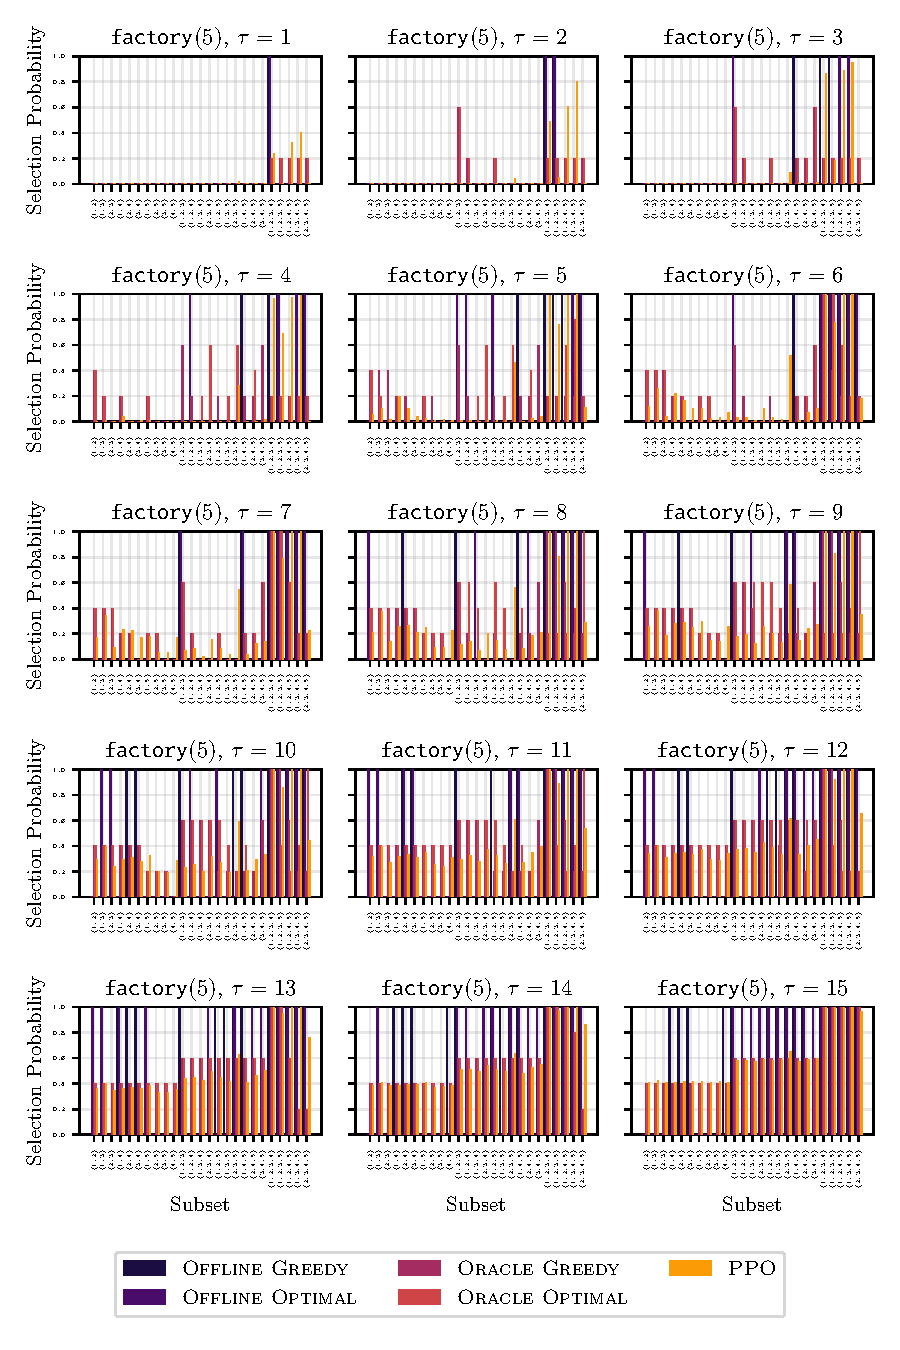
\includegraphics[width=\textwidth]{figures/l2_norm_predictible_factory5_coalition_bars.pdf}
	\caption{ The probability of revealing a given subset for $\tau=1\ldots 15$ for the different approaches, when ran on the $\factory[5]$ distribution with the $ L_2 $-divergence. 
		The resulting divergence can be seen in \Cref{fig:factory}.
	}
\end{figure*}

\begin{figure*}[t!]
  \centering
	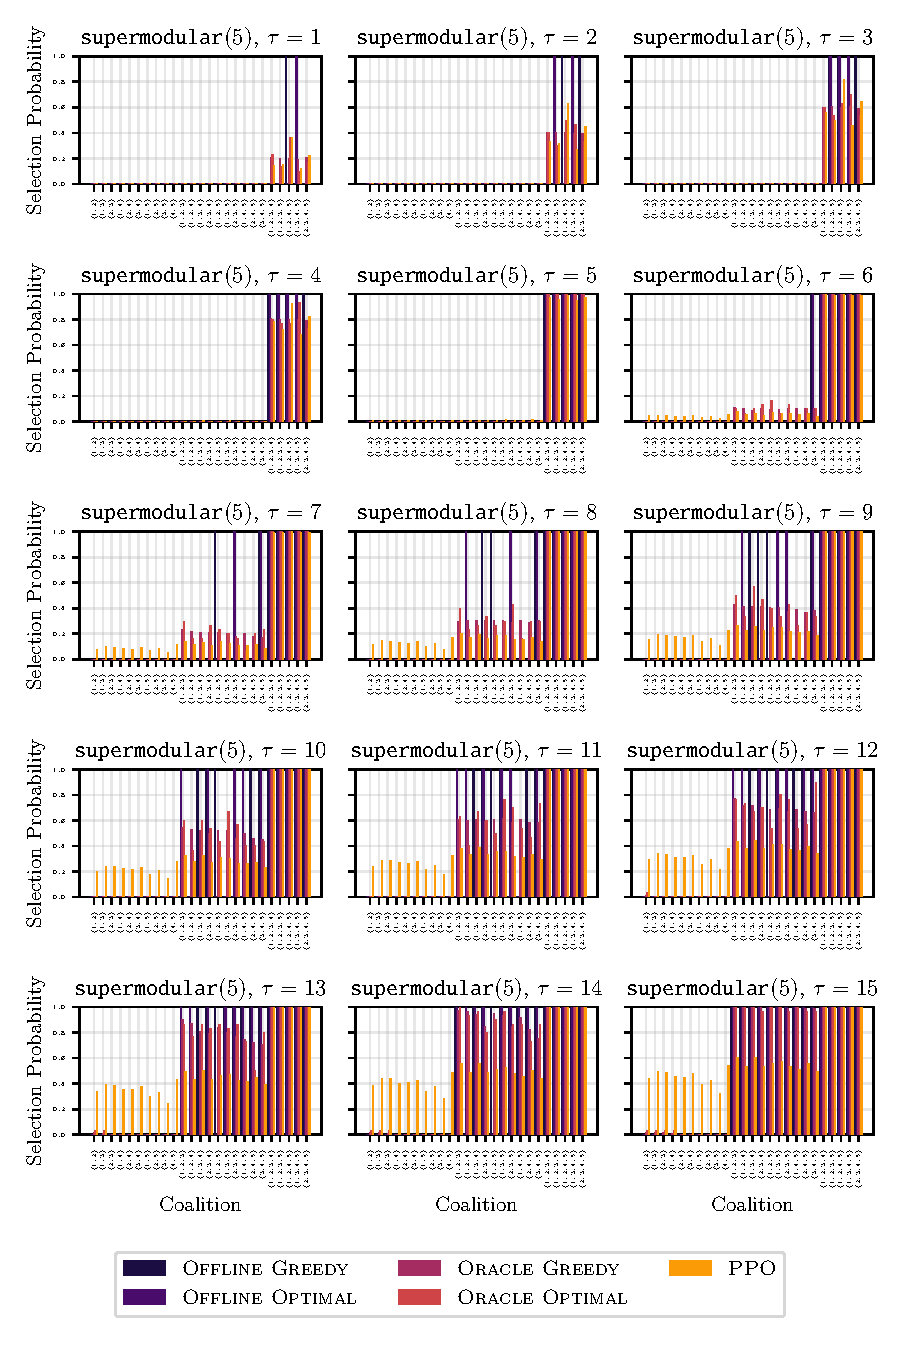
\includegraphics[width=\textwidth]{figures/exploitability_convex5_coalition_bars.pdf}
	\caption{ The probability of revealing a given subset for $\tau=1\ldots 15$ for the different approaches, when ran on the $\supermodular[5]$ distribution with the utopian gap. 
		The resulting utopian gap can be seen in \Cref{fig:supermodular}.
	}
\end{figure*}

\begin{figure*}[t!]
  \centering
	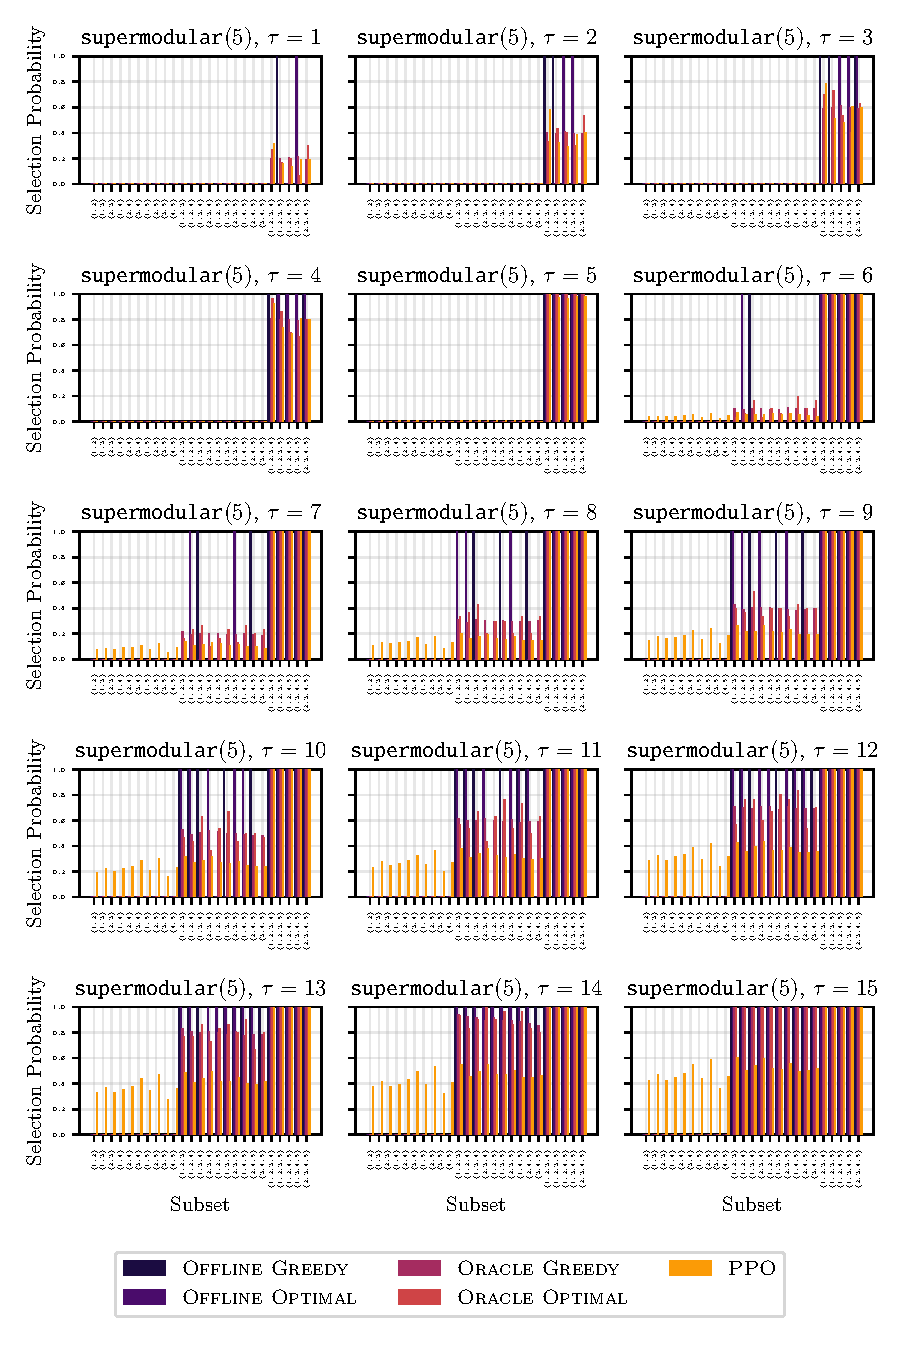
\includegraphics[width=\textwidth]{figures/l1_norm_convex5_coalition_bars.pdf}
	\caption{ The probability of revealing a given subset for $\tau=1\ldots 15$ for the different approaches, when ran on the $\supermodular[5]$ distribution with the $ L_1 $-divergence. 
		The resulting divergence can be seen in \Cref{fig:supermodular}.
	}
\end{figure*}

\begin{figure*}[t!]
  \centering
	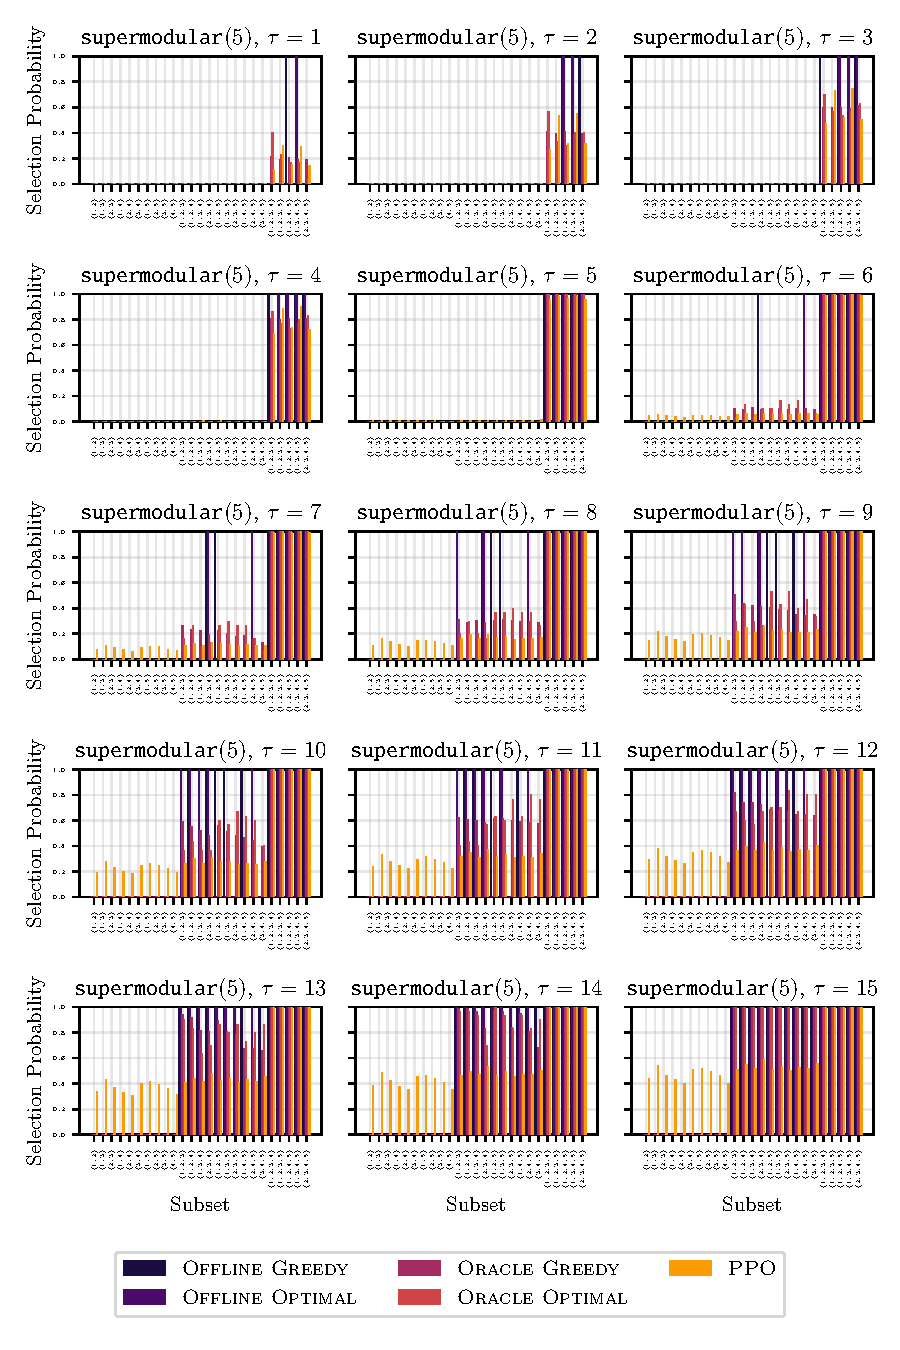
\includegraphics[width=\textwidth]{figures/l2_norm_convex5_coalition_bars.pdf}
	\caption{ The probability of revealing a given subset for $\tau=1\ldots 15$ for the different approaches, when ran on the $\supermodular[5]$ distribution with the $ L_2 $-divergence.
		The resulting divergence can be seen in \Cref{fig:supermodular}.
	}
\end{figure*}

\begin{figure*}[t!]
  \centering
	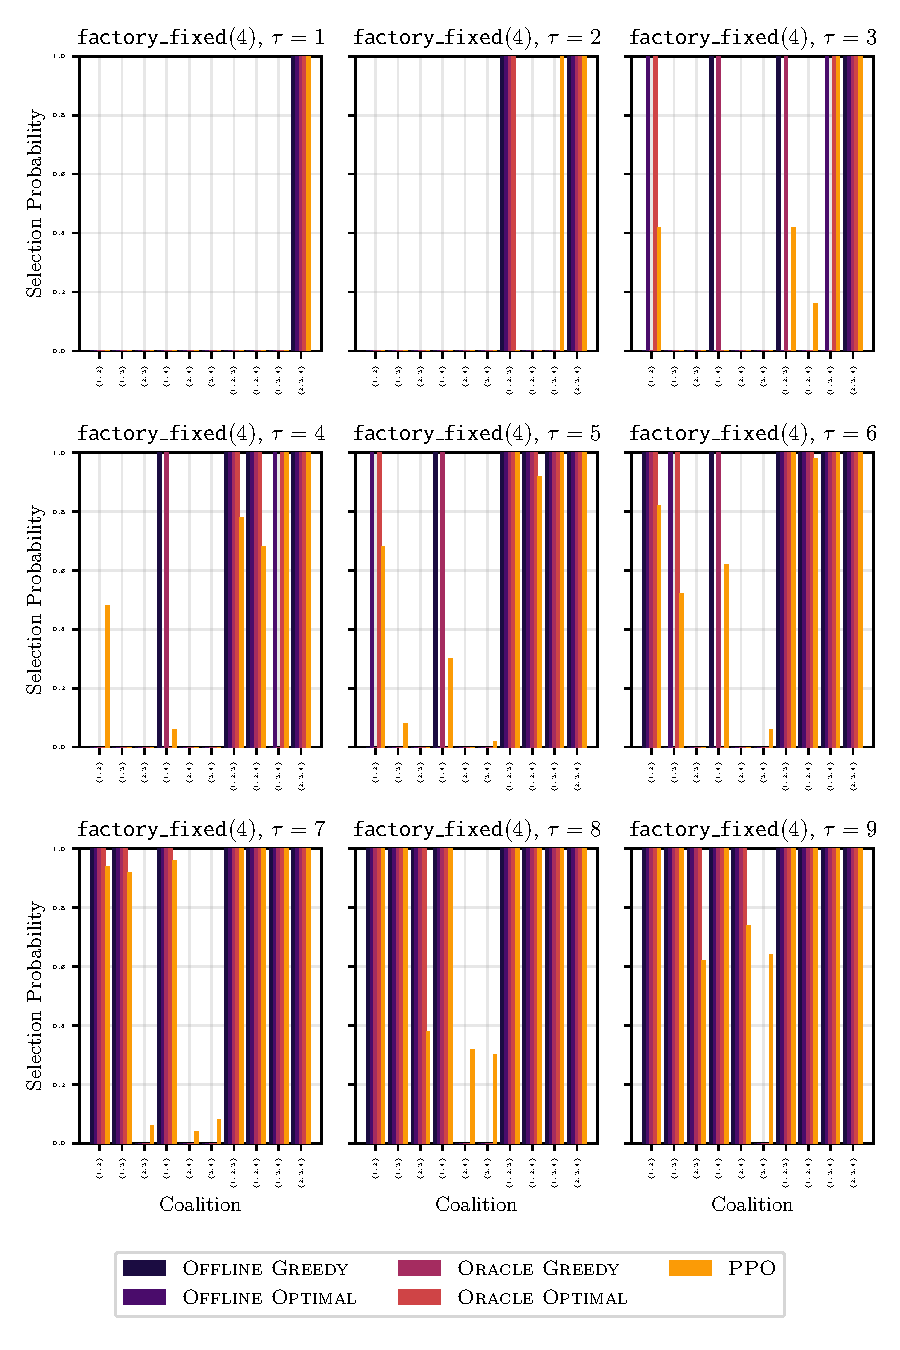
\includegraphics[width=\textwidth]{figures/exploitability_factory_fixed4_coalition_bars.pdf}
	\caption{ The probability of revealing a given subset for $\tau=1\ldots 9$ for the different approaches, when ran on the $\factoryf[4]$ distribution with the utopian gap.
		The resulting divergence can be seen in \Cref{fig:supermodular}.
	}
\end{figure*}
